\documentclass[conference]{IEEEtran}
\IEEEoverridecommandlockouts
% The preceding line is only needed to identify funding in the first footnote.
% If that is unneeded, please comment it out.
%\usepackage[backend=bibtex,style=verbose-trad2]{biblatex}

\usepackage{adjustbox}
\usepackage{algorithmic}
\usepackage{amsmath,amssymb,amsfonts}
%\usepackage[backend=bibtex,style=ieee]{biblatex}
%\usepackage{bookmark}
\usepackage{tabularx,array}
\usepackage{booktabs}
\usepackage{caption}
\usepackage{cite}
\usepackage{color}
\usepackage[inline]{enumitem}
\usepackage{float}
\usepackage[T1]{fontenc}
%\usepackage{fontspec}
\usepackage{svg}
\usepackage{footnote}
\usepackage{graphicx}
\usepackage[colorlinks=true,citecolor=blue]{hyperref}
\usepackage{inputenc}[utf8]
\usepackage{listings}
\usepackage{textcomp}
\usepackage[flushleft]{threeparttable}
\usepackage{subcaption}
\usepackage{xcolor}
\usepackage{cleveref}

\title{OpenCSD: Log Structured Filesystem (LFS) enabled Computational Storage Device platform%\\
%{\footnotesize \textsuperscript{*}Note: Sub-titles are not captured in Xplore
% and should not be used}
%\thanks{Identify applicable funding agency here. If none, delete this.}
}

\pagenumbering{arabic}
\pagestyle{plain}

% Ensure decimal numbering in table  of contents
\renewcommand{\thesection}{\arabic{section}}
\renewcommand{\thesubsection}{\arabic{section}.\arabic{subsection}}
\renewcommand{\thesubsubsection}{\arabic{section}.\arabic{subsection}.\arabic{subsubsection}}

% ensure decimal numbering for sub sections
\makeatletter
\renewcommand{\@seccntformat}[1]{\csname the#1\endcsname.\quad}
\makeatother

% ------------------------------------------------------------------------%
% Proper Python Syntax Highlighting                                       %
% Author: redmode
% https://tex.stackexchange.com/questions/83882/how-to-highlight-python   %
% -syntax-in-latex-listings-lstinputlistings-command#83883                %
% ----------------------------------------------------------------------- %

% Default fixed font does not support bold face
\DeclareFixedFont{\ttb}{T1}{txtt}{bx}{n}{8} % for bold
\DeclareFixedFont{\ttm}{T1}{txtt}{m}{n}{8}  % for normal

% Custom colors
\definecolor{deepblue}{rgb}{0,0,0.5}
\definecolor{deepred}{rgb}{0.6,0,0}
\definecolor{deepgreen}{rgb}{0,0.5,0}

% Python style for highlighting
\newcommand\pythonstyle{
	\lstset{
		language=Python,
		basicstyle=\ttm,
		showstringspaces=false,
		tabsize=4,
		aboveskip=0.2cm,
		belowskip=0.2cm,
		otherkeywords={self},             % Add keywords here
		keywordstyle=\ttb\color{deepblue},
		emph={MyClass,__init__},          % Custom highlighting
		emphstyle=\ttb\color{deepred},    % Custom highlighting style
		stringstyle=\color{deepgreen},
		frame=tb,                          % Any extra options here
		prebreak=\textbackslash,
		linewidth=8.85cm,
		breaklines=true,
	}
}

% Python environment
\lstnewenvironment{python}[1][] {
	\pythonstyle\lstset{#1}
}{}

% Python for inline
\newcommand\pythoninline[1]{{\pythonstyle\lstinline!#1!}}

% Python for external file
\newcommand\pythonexternal[2][]{{\pythonstyle\lstinputlisting[#1]{#2}}}

% ----------------------------------------------------------------------- %

% Bash style for highlighting
\newcommand\bashstyle{
	\lstset{
		language=Bash,
		basicstyle=\ttm,
		showstringspaces=false,
		tabsize=2,
		%commentstyle=itshape,
		aboveskip=0.2cm,
		belowskip=0.2cm,
		prebreak=\textbackslash,
		extendedchars=true,
		mathescape=false,
		% literate= {\$}{{\textcolor{blue}{\$}}}1 {&}{{\textcolor{blue}{\&}}}1 {/n}{{\textcolor{green}{\textbackslash n}}}1,
		linewidth=8.85cm,
		breaklines=true
	}
}

% Bash environment
\lstnewenvironment{bash}[1][] {
	\bashstyle\lstset{#1}
}{}

% Bash for inline
\newcommand\bashinline[1]{{\bashstyle\lstinline!#1!}}

% Bash for external file
\newcommand\bashexternal[2][]{{\bashstyle\lstinputlisting[#1]{#2}}}


% Python style for highlighting
\newcommand\cstyle{
	\lstset{
		language=c,
		basicstyle=\ttm,
		showstringspaces=false,
		tabsize=4,
		aboveskip=0.2cm,
		belowskip=0.2cm,
		otherkeywords={self},             % Add keywords here
		keywordstyle=\ttb\color{deepblue},
		emph={MyClass,__init__},          % Custom highlighting
		emphstyle=\ttb\color{deepred},    % Custom highlighting style
		stringstyle=\color{deepgreen},
		frame=tb,                          % Any extra options here
		prebreak=\textbackslash,
		linewidth=8.85cm,
		breaklines=true,
	}
}

% Python environment
\lstnewenvironment{clist}[1][] {
	\cstyle\lstset{#1}
}{}

% Python for inline
\newcommand\cinline[1]{{\cstyle\lstinline!#1!}}

% Python for external file
\newcommand\cexternal[2][]{{\cstyle\lstinputlisting[#1]{#2}}}

% ----------------------------------------------------------------------- %

\begin{document}

\begin{titlepage}
\begingroup
\centering
{\LARGE\bfseries OpenCSD: Log Structured Filesystem (LFS) enabled Computational Storage Device platform}

\vspace{1cm}

{\Large Vrije Universiteit (VU)}

\vspace{0.5cm}

{Corne Kenneth Lukken}

{\textit{Department of Computer Science} \\
Amsterdam, Netherlands \\
info@dantalion.nl}

\vspace{0.5cm}

\today

\vspace{4.0cm}

\includegraphics[width=0.8\textwidth]{resources/images/loader-pfs-arch-2.drawio.png}

\vfill
\endgroup
\begin{minipage}{0.4\textwidth}
	\begin{tabular}{ll}
		% \Large Thesis: & \Large Log Structured Filesystem for Computational Storage Device \\
		\Large Supervisor: & \Large Animesh Trivedi \\
	\end{tabular}
\end{minipage} \hfill
\begin{minipage}{0.3\textwidth}
	\begin{flushright}
	\includegraphics[width=\textwidth]{resources/images/vu-logo.png}
\end{flushright}
\end{minipage}
\end{titlepage}

\clearpage
\onecolumn

% Ensure black link color in table of contents
\hypersetup{
	linkcolor=black
}

\renewcommand{\contentsname}{CONTENTS}
\tableofcontents{}

\hypersetup{
	linkcolor=blue
}

\twocolumn

\addcontentsline{toc}{section}{\protect\numberline{}INTRODUCTION}
\section*{INTRODUCTION}

% We have a separate previous work section we will ignore most of the different
% related literature in the introduction.

% Problem

The amount of data being generated and processed worldwide is growing rapidly.
Meanwhile the prevelant Von Nuemann computer architecture requires all data is 
moved to system memory before it can be processed\cite{2018-neumann-bottleneck}.
Until recently storage devices such as hard-disk drives (HDDs) or solid state
drives (SSDs) have only been passively storing data. With the increasing
bandwidth persistent storage devices like SSDs achieve this excessive data
movement to memory is increasingly becoming a bottleneck\cite{2014-micro-ndp}.
Similarly, the CPU generational performance
improvements\cite{2016-western-digital} as well as link speeds of interconnects
are stagnating compared to nand flash bandwidth\cite{10.1145/3286588}, the
underlying technology enabling modern SSDs.

% Potential solution and benefits

A promising solution to this problem is the processing of data in-situ by
pushing compute to the storage layer. This solution is actively being researched
as \textit{"Programmable Storage"} and \textit{"Computational Storage"} among
other terms. The concept is not new however, as it has been previously
explored in database mainframes\cite{database-computer} as well as for
conventional HDDs\cite{active-disk-pillar, active-disks-tech, intelligent-disk}.
With rise of Non-Volatile Memory Express (NVMe) technologies offering signifcantly more 
device-internal bandwidth this concept is being revisted. What makes NVMe SSDs
even more suited is that they already contain capable processing units often
boasting even multiple cores. This requirement comes from the internal
management the device has to perform known as the
\textit{Flash Translation Layer} (FTL). Devices utilizing computational elements
on conventional SSDs for \textit{Computational Storage} are commonly known as
\textit{Computational Storage Devices} (CSx)s. The potential benefits of such a
heteregenous architecture offering programmable storage include energy saving,
cost reduction and performance improvements.

% Challenges

Despite all these benefits there is still no widespread adoption even after a
decade of research\cite{lukken2021past}. A multitude of challenges
have prohibited this adoption of which several still applicable today. Four
prominent challenges include that, firstly, \textit{Computational Storage}
requires complete vertical integration. Meaning that changes are required at all
levels of abstraction, device hardware, interfaces, drivers and operating system
to name a few. Trying to integrate a solution for all levels in one prototype
results in a very large problem space. This large problem space complicates
deriving standards for designs and interfaces although the development of such a
standard by SNIA is on-going\cite{snia-model}. Secondly, vendors might choose to
use different hardware with different
\textit{Instruction Set Architectures} (ISA)s or different host-to-device
interfaces. These differences might result in incompatible user applications
across vendors hurting reusability and hindering adoption. Third, filesystems
are managed by the host operating system while the FTL is
managed by the device. Given that one is not aware of the processes within the
other, this semantic gap complicates several aspects such as consistency,
concurreny, multi-user tenancy and filesystem integration. Lastly, no
specialized filesystem designs exist that support both regular user access
concurrent with \textit{Computational Storage} offloading.

% Solutions

In this work we address each of these challenges directly and propose a
complete \textit{Computational Storage} solution that offers a filesystem
capable of concurrent multi-user tenancy with both regular and compute
offloading access (hybrid). We introduce each of the solutions briefly before
describing their complete case. Firstly, we circumvent the complexity of
complete vertical integration by creating a simulation platform on top of
QEMU\cite{qemu}. Secondly, We eliminate potential incompatibities across vendors
by using \textit{Extended Berkely Packet Filer} (eBPF)\cite{what-ebpf} as
compute kernel language. Third, We bridge the semantic gap by using Zoned
Namespaces (ZNS)\cite{zns} SSDs which moves the FTL to the host operating
system (host-managed). Lastly, we allow for concurrent multi-user tenancy in
a \textit{Hybrid Filesystem} context by developing a specialized
\textit{Log-Structured Filesystem} (LFS)\cite{Rosenblum1992TheDA} with an
in-memory snapshot consistency model\cite{Viotti2016ConsistencyIN}. We present
this complete solution as \textit{OpenCSD} an open-source Apache 2 licensed CSx
simulation framework with accompanying filesystem called
FluffleFS\cite{qemu-csd}.

\subsection*{A Case for CSx Simulation}

The lack of a standardized design has lead to a large variety of different
hardware architectures being explored including using embedded CPUs or
\textit{Field-Programmable Gate Arrays} (FPGA)s. Moreover, closed-source
devices have even become commercially available. Still there is a lot of
uncertainty about the right computational hardware models, interconnects and
interconnects their interfaces. Even though the \textit{Peripheral Component
Interconnect Express} (PCIe) interconnect and the NVMe storage interface
currently dominate modern storage devices it is unclear if their current
capabilities are sufficient to support CSxs. Meanwhile existing technologies
such as QEMU allow rapid development of new simulated hardware.

The lack of a clear standardized design combined with the ease of prototyping
designs in simulation clearly shows that choosing simulation over an actual
hardware prototype is the current logical choice.

\subsection*{A Case for eBPF Programmability}

The concept of programmability provides end users the capability to run their
own provided code. With the introduction of modern \textit{Operating Systems}
(OS)s this is expected to happen in safe and dynamic manner. Programmability
can be achieved in different manners such as through the kernel in kernel
modules, with filesystems through \textit{Virtual File System} (VFS) or FUSE and
with language runtimes such as those in Python. In addition programmability can
also target a peripheral instead of the host directly such as is prevelant in
\textit{General-Purpose computing on Graphics Processing Units} (GPGPU)
programming through \textit{Application Programming Interfaces} (API)s like
OpenCL\cite{opencl} and CUDA\cite{cuda}. Through similar mechanisms
programmability in CSxs can be achieved.

The uncertainty of the hardware design makes it unclear exactly how close to the
hardware and through which method of programmability CSxs will be effective.
Although, naturally, the closer to the actual storage the better
(Near-Data Processing). Therefor, our programmability must not be restricted or
favor a particular type.

Introducing eBPF an ISA and API with a large collection of toolchains and
wideranging implementations\cite{what-ebpf, McCanne1993TheBP}. These
implementations range from complex such as the one found in the Linux kernel to
simple such as the one found in uBPF\cite{ubpf}, with the key difference in
complexity being the supported API. Effectively, the implementation running
(runtime) eBPF code decides the API by tying special eBPF syscall instructions
to predefined code. In addition, this allows the user program and runtime to
exchange important information such as prominently done in Linux through eBPF
maps\cite{bpf-man}.

The benefits of eBPF are four fold. First, the ISA is not tailored to any
specific domain and it has been used in networking\cite{xdp},
tracing\cite{enhanced-ebpf} and security\cite{seccomp} applications. Second,
the simple nature of the eBPF ISA allows for verification and bounded execution
checking such as performed by the Linux kernel\cite{kern-analysis}. Third, eBPF
supports efficient code generation through jitting achieving close to bare-metal
performance. Lastly, eBPF has been positioned as the unified ISA for
heteregenous computing\cite{Brunella2020hXDPES, bpf-uapi}.

\subsection*{A Case for ZNS}

A new emerging NVMe standard is Zoned Namedspaces (ZNS). It can been seen as the
technical successor to Open-Channel\cite{}. This standard allows host visibility
and control over data placement (host-managed) while more closely representing
nand flash behavior. This replacement for the traditional block interface offers
reduced write-ampplifcation, lower SSD hardware requirements and more
intelligent wear-leveling and garbage collection. However ZNS SSDs come with
several constraints such as not allowing in-place updates (append-only), using a
large collection of sectors as single erasure unit and requiring wear-leveling
and garbage collection to be explicitly programmed by the host.

Yet we argue ZNS greatly improves the feasibility of CSx supporting
\textit{hybrid filesystems}. Firstly, ZNS offers more predictable performance in
conjuction with \textit{Log-Structured Filesystems} as the absence of an FTL
means the behavior of \textit{append-only} writes won't be influenced by
underlying write-amplification or garbage-collection. Secondly, the direct
relationship between dimensions as reported to the host and to those known on
the device results in a greatly simplified exchange of information from host
submitted compute kernels as well as reduced kernel runtime translations.
Finally, this reduced semantic gap between the host and device is essential to
compute kernels running autonomously and without shared virtual memory.

\subsection*{A Case for LFS}

\textit{Log-Structured Filesystems} have been around for a long
time\cite{Rosenblum1992TheDA} but have not really been popularized until the
recent advancement of nand flash. A LFS maintains one or multiple logs which
are append-only sections of the filesystem. This has the advantage of the
underlying device receiving filesystem writes as sequential I/O operations,
which is known to improve performance. In addition, LFSs are often relatively
easy to implement. Unfortunately, LFSs suffer from write-amplification because
modifcations updating inode or other data location information travels up the
chain in history.

Yet we argue an LFS is essential for an effective \textit{hybrid filesystem} due
to the following three reasons. Firstly, the append-only nature of a LFS is the
best fit for the append-only requirement of ZNS SSDs. Secondly, the
chronological order of logs allow for snapshotting, versioning and simplified
crash recovery. It is thanks to the properties of an LFS that FluffleFS is able
to provide in-memory snapshots to compute kernels. Lastly, the problem around
write-amplification is a solved issue thanks to the F2FS\cite{Lee2015F2FSAN}
work which introduced so called Node Address Tables (NAT).

\section{Previous Work}

While OpenCSD is unique it is by no means the first CSx prototype as there
has been over a decade of research in this field\cite{lukken2021past}. In this
decade we have seen a large variety of approaches, problem spaces, hardware
platforms and software APIs. While this decade of research shows overall
progression several important challenges are still open research
questions\cite{barbalacecomputational}.

In this section we first introduce characterstics of CSx prototypes such as the
hardware platform and software API. Secondly, introduce the most prominent open
research questions in CSx research. Third, provide an overview of notable works
of the past decade. Fourth, describe the general progression of the field across
these works. Lastly, describe fundamentally missing features that hinder
adoption and widespread use of CSxs.

% Introduce early working prototypes

% Demonstrate different hardware platforms, embedded CPU, vs FPGA.

% List of BPF using storage literature (Blockndp:, Extos: Data-centric
%extensible os, Ex-tension framework for file systems in user space, 
%  Safe and efficient remote application code execu-tion on disaggregated NVM,
% BPF for storage: an exokernel-inspired approach )

% Introduce previous ZCSD table but extended

\subsection{CSx characterstics}

\begin{enumerate}
    \item Bistream; bitstream programmed directly unto FPGA.
    \item Embedded; single program, single memory space, no OS just 'real mode'.
    \item Accelerators; OpenCL, Vulkan.
    \item Real-Time operating system;
    \item Operating System;
    \item Container;
    \item Virtual Machine;
\end{enumerate}

The degree of programmability can be categorized as follows.

\begin{enumerate}
    \item Transparent operations, (de)compression (Playstation 5 I/O Controller)
    \item Fixed functions, unchangeable, workload specific \cite{2013-fast-active-flash}
    \item Fixed function dataflow programming \cite{Wickremesinghe02distributedcomputing}
    \item Query offloading, SQL, NoSql, Regex \cite{10.14778/2994509.2994512}
    \item Event driven (hooks) user-programmable functions \cite{10.1145/3429357.3430519}
    \item Arbitrary code execution, VHDL, eBPF, TCL \cite{10.1145/605432.605425, kourtis2020safe}
\end{enumerate}

\onecolumn

\begin{table}[H]
    \caption{Programmable flash storage overview}
    \centering
    \begin{adjustbox}{width=1\textwidth}
        \begin{threeparttable}[]
            \begin{tabular}{lllll}
                \toprule
                \textbf{Name} & \textbf{Programmability} & \textbf{Programming Model} & \textbf{Interface} & \textbf{CSEE} \\
                \midrule
                Active SSD \cite{6062973} & Event driven & Dataflow (streams) & PCIe & Operating system (Custom) \\
                Smart SSD \cite{6558444} & Event driven & Dataflow (MapReduce) & SATA & Embedded \\
                Smart SSD \cite{10.1145/2463676.2465295} & Event driven & Shared memory & SATA & Embedded \\
                Intelligent SSD \cite{10.1145/2464996.2465003, 10.1145/2505515.2507847} & Arbitrary code execution\footnotemark[7] & Shared memory\footnotemark[7] & N.A. & Operating system (Linux)\footnotemark[7] \\
                Ibex \cite{10.14778/2732967.2732972} & Query offloading (MySQL) & Declarative & SATA & Bitstream \\
                Willow \cite{186149} & Arbitrary code execution & Client / Server (RPC) & PCIe (NVMe) & Operating system (Custom) \\
                Biscuit \cite{2016-isca-biscuit} & Event driven & Dataflow & PCIe & Embedded \\
                Hadoop ISC* \cite{7524716} & Event driven & Dataflow (MapReduce) & SAS & Embedded \\
                YourSQL \cite{10.14778/2994509.2994512} & Query offloading (MySQL) & Declarative & PCIe (NVMe) & Bitsream\footnotemark[8] \\
                Summarizer \cite{10.1145/3123939.3124553} & Event driven & Shared memory & PCIe (NVMe) & Embedded \\
                NDP RE2 regex* \cite{10.1145/3211922.3211926} & Query offloading (Regex) & N.A. & N.A. & Embedded \\
                Registor \cite{10.1145/3310149} & Query offloading (Regex) & Shared memory & PCIe (NVMe) & Bitsream \\
                Cognitive SSD \cite{8839401} & Arbitrary code execution & Shared memory & PCIe (NVMe, OpenSSD) & Accelerators (Custom) \\
                INSIDER \cite{234968} & Event driven & Shared memory (VFS) & PCIe & Bitstream \\
                Catalina \cite{8855540} & Arbitrary code execution & Client / Server (MPI) & PCIe (NVMe) & Operating system (Linux) \\
                THRIFTY \cite{10.1145/3400302.3415723} & Event driven\footnotemark[9] & Shared memory (VFS)\footnotemark[9] & PCIe\footnotemark[9] & Bitstream\footnotemark[9] \\
                POLARDB \cite{246154} & Query offloading (POLARDB) & Declarative & PCIe & Bitstream \\
                NGD newport \cite{10.1145/3415580} & Arbitrary code execution & Client / Server & PCIe (NVMe) & Operating system (Linux) \\
                blockNDP \cite{10.1145/3429357.3430519} & Event driven & Dataflow (streams) & PCIe (NVMe, OpenSSD) & Virtual Machine (QEMU) \\
                QEMU CSD* \cite{10.1145/3439839.3459085} & Arbitrary code execution & Shared memory & PCIe (NVMe) & N.A. (Simulated) \\
                \bottomrule
            \end{tabular}
            \begin{tablenotes}[para,flushleft]
                \centering Overview of PFS works and various aspects as
                    previously detailed.
            \end{tablenotes}
        \end{threeparttable}
        \label{table:pfsoverview}
    \end{adjustbox}
\end{table}

\twocolumn

\section{Research Questions}

How to achieve multi-user tenancy in a Log Structured Filesystem (LFS) while
supporting Computational Storage offloading?

What would a Zoned Namespaces (ZNS) Log Structured Filesystem (LFS) look like?

How to register Computational Storage Device (CSx) compute kernels using
existing operating system APIs?

How to differentiate individual users, files and I/O operations in relation to
their CSx compute kernel?

\section{Design}

\subsection{Framework}

% Diagram with overview of different modules and their used as well as
% relationships. Also show integration of open-source technologies.

\begin{figure}
    \centering
	\label{figure:moduledependencies}
	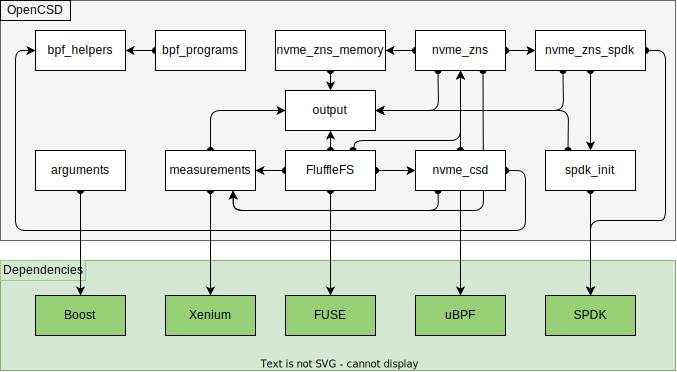
\includegraphics[width=0.5\textwidth]{resources/images/module-dependencies.pdf}
	\caption{Overview of all OpenCSD components and their depends-on relations}
    % \includesvg[width=0.6\columnwidth]{resources/images/module-dependencies}
\end{figure}

\subsection{Filesystem}

% Two write pointers, one for RANDOM ZONE and one for LOG ZONE. Use of ZNS is
% optional but allows for lower write-amplification and more explicit garbage
% collection

\subsubsection{Concurrency}

\subsection{Offloading}

% Filesystem extended attributes, PID + INODE

\section{implementation}

\section{Considerations}

\subsection{Filesystem}

% Filesystem does not restore in-memory datastructures upon mounting the
% filesystem making it non-persistent. Can be achieved through NAT and SIT
% blocks.

% Fsync, rename, unlink, rmdir, listxattr and removexattr are unimplemented.

% No ACL, all files / directories appear to have the caller as owner / group.

\subsection{Interface}

% Maximum 128Kb stride due to kernel, make diagram of how the arguments for
% this system call are parsed.

% Stream kernels can not return more data than the size of the snapshotted file.
% Stream kernels can not return more data than specified in the read request.

% Event kernels can not return any data?

% Mtime modifications to prevent FUSE internal caches with snapshots.

\subsection{Offloading}

% Safety

\section{Evaluation}

\subsection{Filtering}

\subsection{Entropy}

\subsection{Indexing}

% \footnotemark[1]

% \footnotetext[1]{Time of writing is $10^{th}$ of February 2021.}

% \begin{center}
% 	\begin{figure}[H]
% 		\bashexternal{resources/bash/gitmodules.sh}
% 		\captionsetup{justification=centering}
% 		\caption{Contents of \textit{.gitmodules} file for this project.}
% 		\label{fig:example-gitmodules}
% 	\end{figure}
% \end{center}

% \begin{table}[h!]
% 	\caption{BPF resources and their relevance}
% 	\label{table:bpfresources}
% 	\centering
% 	\begin{adjustbox}{width=0.5\textwidth}
% 		\begin{threeparttable}[]
% 			\begin{tabular}{lllll}
% 				\toprule
% 				\textbf{Resource} & \textbf{Category} & \textbf{Value} &
% 				\textbf{Length} & \textbf{Age} \\
% 				\midrule
% 				\href{https://www.man7.org/linux/man-pages/man2/bpf.2.html}{Linux bpf manpage}\cite{bpfman} &
% 				Linux Kernel & medium & short & timeless \\
% 				\href{https://www.kernel.org/doc/Documentation/networking/filter.txt}{BPF kernel documentation}\cite{Linuxbpf} &
% 				Linux Kernel & low & long & outdated \\
% 				\href{https://www.kernel.org/doc/html/latest/bpf/btf.html}{Linux BTF documentation}\cite{Linuxbtf} &
% 				Linux Kernel \& BTF & low & medium & timeless \\
% 				\href{https://facebookmicrosites.github.io/bpf/blog/2020/02/19/bpf-portability-and-co-re.html}{BPF portability and CO-RE}\cite{bpfport} &
% 				BPF CO-RE \& BTF & high & medium & relevant \\
% 				\href{https://nakryiko.com/posts/libbpf-bootstrap/}{BPF applications with libbpf-bootstrap}\cite{bpfapplications} &
% 				libbpf - libbpf-bootstrap & high & short & relevant \\
% 				\href{https://www.oreilly.com/library/view/linux-observability-with/9781492050193/}{Linux Observability with BPF}\cite{observabilityoreilly} &
% 				libbpf - bpf\_load & medium & book & outdated \\
% 				\href{https://facebookmicrosites.github.io/bpf/blog/2020/02/19/bpf-portability-and-co-re.html}{Cilium BPF + XDP reference guide}\cite{ciliumbpf} &
% 				libbpf & high & long & relevant \\
% 				\href{https://facebookmicrosites.github.io/bpf/blog/2020/02/20/bcc-to-libbpf-howto-guide.html}{BCC to libbpf conversion}\cite{libbpfconversion} &
% 				libbpf & low & long & relevant \\
% 				\href{https://github.com/iovisor/ubpf}{uBPF}\cite{ubpf} &
% 				execution / interpretation & medium & short & relevant \\
% 				\href{https://github.com/generic-ebpf/generic-ebpf}{generic-ebpf}\cite{generic-ebpf} &
% 				execution / interpretation & medium & short & relevant \\
% 				\bottomrule
% 			\end{tabular}
% 			\begin{tablenotes}[para,flushleft]
% 				\centering List of resources on BPF and its various elements.
% 			\end{tablenotes}
% 		\end{threeparttable}
% 	\end{adjustbox}
% \end{table}

\section{Future Work} \label{future}

%\footnotemark[1]. example\ref{term}.
%\footnotetext[1]{test}
%\subsection*{Accelerated Computing Landscape}
%\textit{C++}
%GPUOCelot\cite{tired-manycore-architectures-ocelot}
%\section{LARGER SECTION}
%$\mathcal{O}(N\log N)$
%
%\begin{center}
%	\begin{figure}[H]
%		\bashexternal{resources/bash/inxi.sh}
%		\captionsetup{justification=centering}
%		\caption{Output of inxi showing both CPU and GPU hardware configuration}
%		\label{fig:inxihardware}
%	\end{figure}
%\end{center}

%\cite{Rius1995,Karp1996,parreverse,Adikaram2014}.

%\begin{center}
%	\begin{figure}[H]
%		\cexternal{resources/c/basic.c}
%		\captionsetup{justification=centering}
%		\caption{First basic kernel}
%		\label{fig:base}
%	\end{figure}
%\end{center}

\addcontentsline{toc}{section}{\protect\numberline{}TERMINOLOGY}
\section*{TERMINOLOGY} \label{term}

% \begin{tabularx}{\textwidth}{@{}l<{ -}@{\ }X@{}}
% 	ZNS & Zoned Namespace \\
% 	CSD & Computational Storage Device \\
% 	Upstream & {When a certain patch or feature has been merged \\ into the main
% 		repository of a project. }\\
% \end{tabularx}

\begin{enumerate}
	\item HDD - hard-disk drive % 233
	\item SSD - solid state drive % 234
	\item Programmable Storage % 246
	\item Computational Storage % 246
	\item NVMe - Non-Volatile Memory Express % 250
	\item FTL - Flash Translation Layer % 255
	\item CSx - Computational Storage Device % 257
	\item ISA - Instruction Set Architecture % 274
	\item eBPF - Extended Berkely Packet Filter %293
	\item ZNS - Zoned NameSpaces % 294
	\item Host Managed %296
	\item Hybrid Filesystem % 296
	\item LFS - Log-Structured Filesystem % 297
	\item FPGA - Field-Programmable Gat Array % 306
	\item PCIe - Peripheral Component Interconnect Express % 310
	\item OS - Operating System %324
	\item VFS - Virtual File System % 326
	\item GPGPU - General-Purpose computing on Graphics Processing Units % 329
	\item API - Application Programming Interface %330
	\item NAT - Node Address Table % 406
\end{enumerate}

\addcontentsline{toc}{section}{\protect\numberline{}REFERENCES}
\bibliographystyle{IEEEtran}
\phantomsection
\bibliography{bibliography}

\end{document}